\documentclass[12pt,a4paper, pink]{bbe}
\usepackage{blindtext}
\usepackage{listings}
\usepackage{xcolor}
\usepackage{subfiles}
\usepackage{hyperref} %for Hyperlinks

\definecolor{codegreen}{rgb}{0,0.6,0}
\definecolor{codegray}{rgb}{0.5,0.5,0.5}
\definecolor{codepurple}{rgb}{0.58,0,0.82}
\definecolor{codebackcolour}{rgb}{0.95,0.95,0.92}

  	
%added be me.
%Code listing style named "mystyle"
\lstdefinestyle{mystyle}{
    backgroundcolor=\color{codebackcolour},
    commentstyle=\color{codegreen},
    keywordstyle=\color{blue},
    numberstyle=\tiny\color{codegray},
    stringstyle=\color{codepurple},
    basicstyle=\ttfamily\footnotesize,
    breakatwhitespace=false,         
    breaklines=true,                 
    captionpos=b,                    
    keepspaces=true,                 
    numbers=left,                    
    numbersep=5pt,                  
    showspaces=false,                
    showstringspaces=false,
    showtabs=false,                  
    tabsize=2
}

\lstset{style=mystyle}

\begin{document}
    \setcounter{chapter}{9}
	\chapter{Common Algorithms}
	
	
	\section{Linear Search}
	
	If you are trying to find a playing card in a shuffled deck you have to go through them in order to find the one you want. This is a linear search.
	
	\vspace{1cm}
	
	\begin{figure}[h]
        \centering
        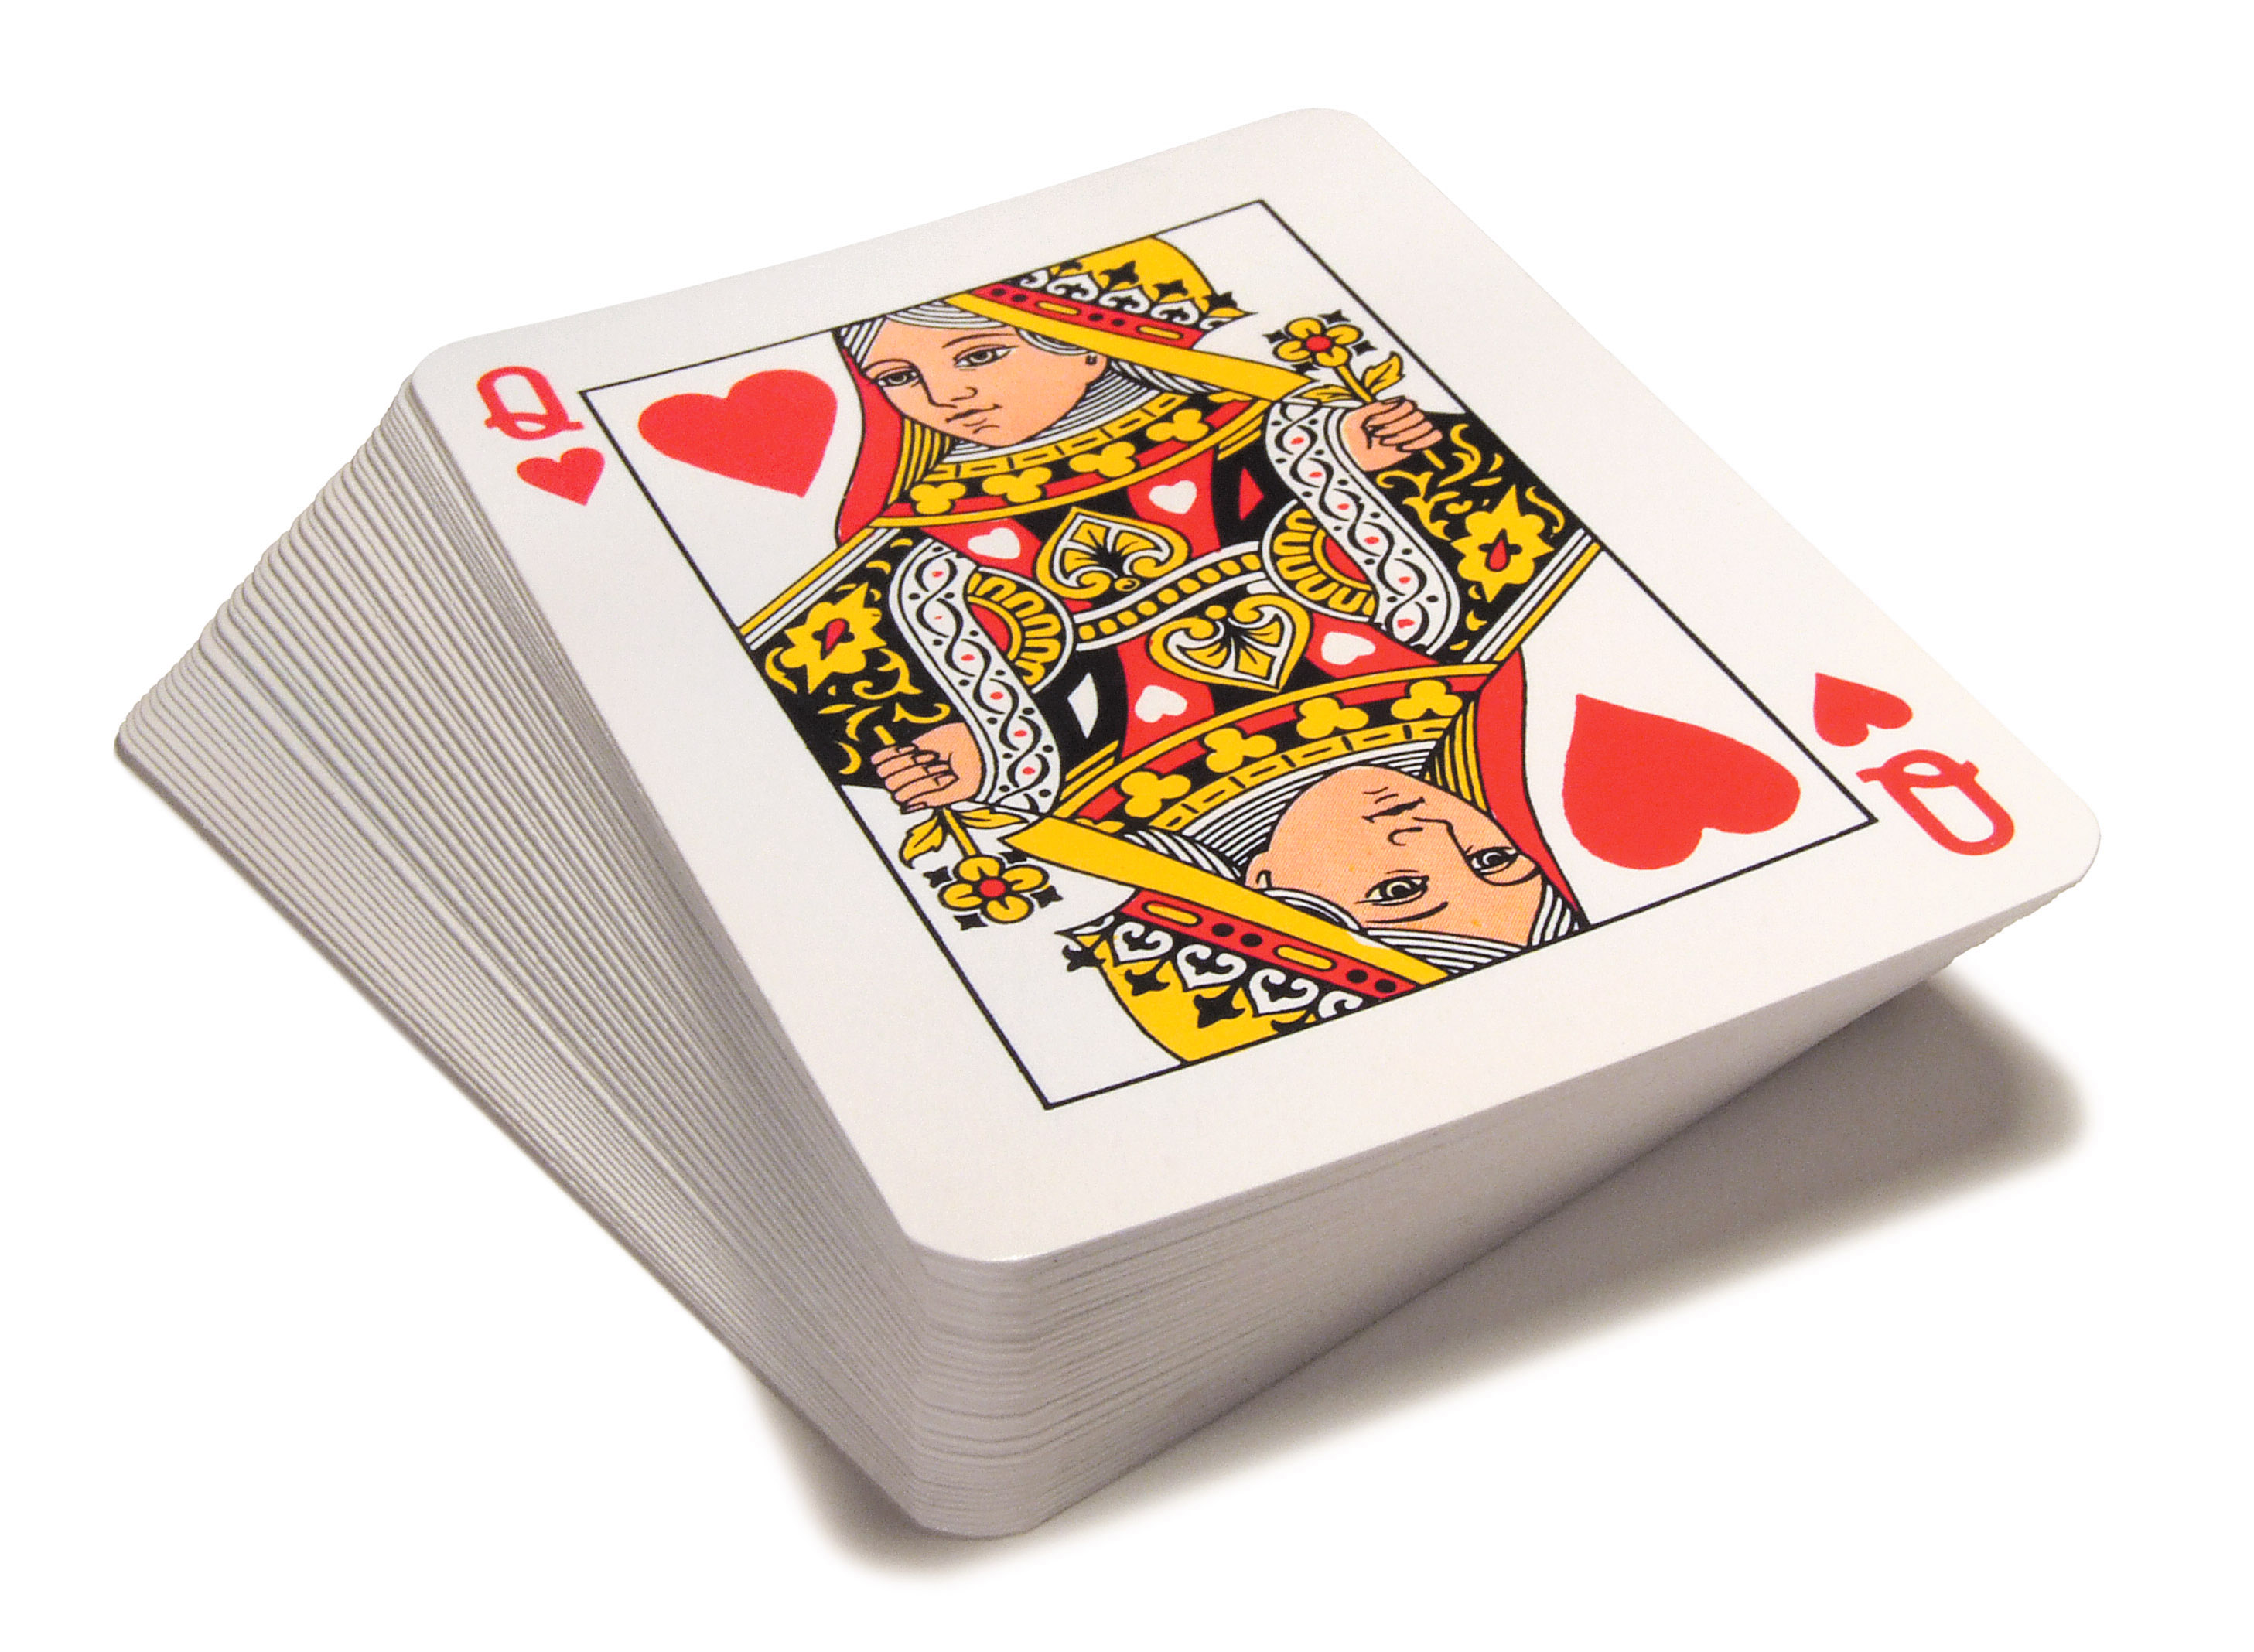
\includegraphics[width=0.4\textwidth]{images/ch9/cards.jpg}
        \caption{Searching a deck of cards}
        \label{fig:mesh1}
    \end{figure}
    \vspace{5mm}
    
We may wish to search the list below for the number 7. To do this we would start at element 0, and then move to element 1, 2, 3 and so on. Each time checking if this element contains 7. On the 9th search (element 8) we find our number.
\vspace{5mm}
    
% Please add the following required packages to your document preamble:
% \usepackage[table,xcdraw]{xcolor}
% If you use beamer only pass "xcolor=table" option, i.e. \documentclass[xcolor=table]{beamer}

\begin{table}[h]
\centering
\begin{tabular}{|l|l|l|l|l|l|l|l|
>{\columncolor[HTML]{CBCEFB}}l |l|}
\hline
\textbf{0} & \textbf{1} & \textbf{2} & \textbf{3} & \textbf{4} & \textbf{5} & \textbf{6} & \textbf{7} & \textbf{8} & \textbf{9} \\ \hline
2          & 5          & 8          & 3          & 20         & 16         & 0          & 9          & 7          & 12         \\ \hline
\end{tabular}
\end{table}

	
 \vspace{5mm}
 
    This search will work on unsorted data as it goes over every element until its found. This means it may have to look at every element - the worst case. Of course it may find it immediately.
    As the number of elements increases - so does the number of average searches needed.
    Imagine a list of 1 million people. On average you may have to search 500 000 to find the person you are searching for.
    
    
    
		
	\section{Binary Search}
	
	
		
	\section{Bubble Sort}
	
	Many tasks require data to be sorted into order. This could be a list of names in alphabetical order or values in data. For example a 2d game engine might sort sprites in depth order before rendering them to the screen.
	
	This common task can be achieved with several different algorithms. Bubble sort is a well know method. It might be relatively slow when you have a lot of data, but it relatively easy to implement. This makes it a good choice in many situations and is worth knowing.
	
	The main idea of bubble sort is that the large numbers will 'bubble up' to the end one at a time.
	\vspace{1cm}
	\lstinputlisting[language=Python]{python/bubble.py}
	
    The output from the programe:
	
	\begin{lstlisting}
    > [1, 2, 3, 4, 5, 6, 7]\end{lstlisting}
   \vspace{1cm}
   
  
   
 
   
   %https://www.tablesgenerator.com/#
% Please add the following required packages to your document preamble:
% \usepackage[table,xcdraw]{xcolor}
% If you use beamer only pass "xcolor=table" option, i.e. \documentclass[xcolor=table]{beamer}
\begin{table}[h]
\begin{tabular}{l|l|l|l|l|l|l|l
>{\columncolor[HTML]{9AFF99}}l l}
\cline{1-7}
\cellcolor[HTML]{FFCCC9}4 & \cellcolor[HTML]{FFCCC9}2 & 5                         & 3                         & 1                         & 7                         & 6                         &  & 1 & The fist and second are compared, and swapped as 4 \textgreater 2 \\ \cline{1-7}
\multicolumn{1}{|l|}{2}   & \cellcolor[HTML]{CBCEFB}4 & \cellcolor[HTML]{CBCEFB}5 & 3                         & 1                         & 7                         & 6                         &  & 2 & The second and third are compared and remain the same             \\ \cline{1-7}
\multicolumn{1}{|l|}{2}   & 4                         & \cellcolor[HTML]{FFCCC9}5 & \cellcolor[HTML]{FFCCC9}3 & 1                         & 7                         & 6                         &  & 3 & The third and fourth are swapped  as 5 \textgreater 3             \\ \cline{1-7}
\multicolumn{1}{|l|}{2}   & 4                         & 3                         & \cellcolor[HTML]{FFCCC9}5 & \cellcolor[HTML]{FFCCC9}1 & 7                         & 6                         &  & 4 & 5 \textgreater 1 so they are swapped                              \\ \cline{1-7}
\multicolumn{1}{|l|}{2}   & 4                         & 3                         & 1                         & \cellcolor[HTML]{CBCEFB}5 & \cellcolor[HTML]{CBCEFB}7 & 6                         &  & 5 & The fifth and sixth remain the same as 5 \textless 7              \\ \cline{1-7}
2                         & 4                         & 3                         & 1                         & 5                         & \cellcolor[HTML]{FFCCC9}7 & \cellcolor[HTML]{FFCCC9}6 &  & 6 & 7 \textgreater 6 so the swap.  The 7 will now be sorted !         \\ \cline{1-7}
\end{tabular}
\end{table}

 \vspace{1cm}
  The above trace table shows the first loop, where the largest number will bubble to the end and is sorted. The loop will now run again and sort the next largest number(6). This will happen 4 more times until all the numbers are in order.
  
  \begin{tracetable}
    A Trace table is used to track the value of variables in the program as they change as the algorithm progresses. This helps you determine the output of the program.
  \end{tracetable}
  
  \begin{recap}
  \vspace{5mm}
	\begin{itemize}[c]
	    \item Linear Search - Search one item at a time in a list
	    \item Binary Search - Half the search space each time, finding items in a sorted list
	    \item Bubble Sort - A simple method for sorting data into order
	    
	\end{itemize}
	
	   Being able to search and sort data are important in many real world tasks. These are important concepts to learn and master.
	\end{recap}
  

\end{document}

